\documentclass[10pt,onecolumn]{article}

\usepackage[margin=1in,top=0.8in,bottom=0.8in]{geometry}
\usepackage{times}
\usepackage{booktabs}
\usepackage{graphicx}
\usepackage{amsmath}
\usepackage{amssymb}
\usepackage{microtype}
\usepackage{caption}
\usepackage{enumitem}
\usepackage{parskip}

\setlength{\parskip}{4pt}
\setlength{\parindent}{0pt}

\title{
    \Large\textbf{GRAFT: Grounded Region-Augmented Fine-Tuning}\\[4pt]
    \large Intermediate Progress Report --- TTIC 31280, Spring 2026
}

\author{
    Siddharth Raj \quad Aniket Agrawal \\
    Toyota Technological Institute at Chicago \\
    \texttt{\{sidraj, aniket\}@ttic.edu}
}

\date{May 14, 2026}

\begin{document}

\maketitle
\thispagestyle{empty}

\textbf{Abstract.}
This report summarises progress on \textbf{GRAFT} (Grounded Region-Augmented
Fine-Tuning), a project aimed at improving patch-level spatial grounding in
SigLIP by fine-tuning with explicit region-level supervision derived from
human-annotated and automatically generated phrase--bounding-box pairs.
We report (a) the current status of experiments, (b) all baseline benchmarking
completed to date, and (c) a revised evaluation design and scope relative to the
original proposal.

\hrule
\vspace{6pt}

\textbf{Models and methods.}
This project uses two distinct vision-language models and one patch-extraction
technique, which appear together throughout the report.
\textbf{CLIP} (Radford et al., 2021) is a contrastive vision-language model
trained with a standard softmax loss; we use the ViT-B/16 variant as a reference
baseline.
\textbf{SigLIP} (Zhai et al., 2023) is a more recent model trained with a sigmoid
pairwise contrastive loss over MHAP-pooled global representations; SigLIP-B/16-384
is the backbone we fine-tune in GRAFT.
\textbf{MaskCLIP} (Ding et al., 2022) is not a separate model but a
\textit{patch-extraction technique}: it replaces the final self-attention layer
of any vision transformer with a value-only projection, bypassing the attention
aggregation and exposing per-patch features that are spatially structured enough
for zero-shot segmentation. We apply this same technique to both CLIP and SigLIP
for all patch-level evaluations. In the VOC table below, ``MaskCLIP'' and
``SCLIP'' are variants of this extraction applied to the CLIP backbone; ``B0'' is
the same extraction applied to our SigLIP backbone before any fine-tuning.

%-----------------------------------------------------------------------
\section{Experiment Status}
%-----------------------------------------------------------------------

\subsection{Completed}

\textbf{Evaluation harness.}
We implemented the MaskCLIP-style last-attention bypass described above,
applied uniformly to all backbone evaluations. All baselines reported in
Section~\ref{sec:findings} use this extraction method.

\textbf{Training pipeline.}
The full fine-tuning pipeline (\texttt{graft-training.ipynb}) applies Low-Rank
Adaptation (LoRA; $r{=}4$, $\alpha{=}16$, targets \texttt{q\_proj} and
\texttt{v\_proj}) to SigLIP-B/16-384, leaving 99.86\% of parameters frozen
(294,914 trainable out of 203.7M total). The training objective is:
\begin{equation*}
    \mathcal{L}_\text{total} = \mathcal{L}_\text{global} + \lambda\,\mathcal{L}_\text{region}
\end{equation*}
where $\mathcal{L}_\text{global}$ is the SigLIP sigmoid contrastive loss and
$\mathcal{L}_\text{region}$ is a FILIP-style patch--token alignment loss.
The dataset loader processes Flickr30k Entities (29,000 training images,
$\sim$12 phrase--bbox pairs per image). The pipeline includes gradient
checkpointing, mixed-precision training, and Weights \& Biases logging.

\textbf{Dataset pivot.}
Following discussion, we pivoted from the originally proposed CC3M subset to
\textbf{Flickr30k Entities}. CC3M was dropped because (1) the 20--30 A100-hours
required for Qwen2-VL-2B inference over 50--100k crops is not feasible in the
remaining timeline, and (2) Flickr30k Entities provides human-annotated
phrase--bbox supervision, giving a clean upper-bound condition
(M$_\text{human}$) against which any auto-labelling method can be compared.

\textbf{Auto-supervision with Florence-2.}
We identified \textbf{Florence-2} (Microsoft, 231M parameters) as the
automatic annotation source. Its \texttt{<DENSE\_REGION\_CAPTION>} task produces
localised bounding boxes with short natural-language labels in a single forward
pass --- exactly the (bbox, phrase) format consumed by
$\mathcal{L}_\text{region}$. A local pilot on five Flickr30k images
(\texttt{05a\_florence2\_auto\_bbox.ipynb}) confirmed qualitatively good
localisation (Figure~\ref{fig:florence2}). Florence-2 will generate the
M$_\text{auto}$ training annotations across the full Flickr30k training split.

\begin{figure}[h]
    \centering
    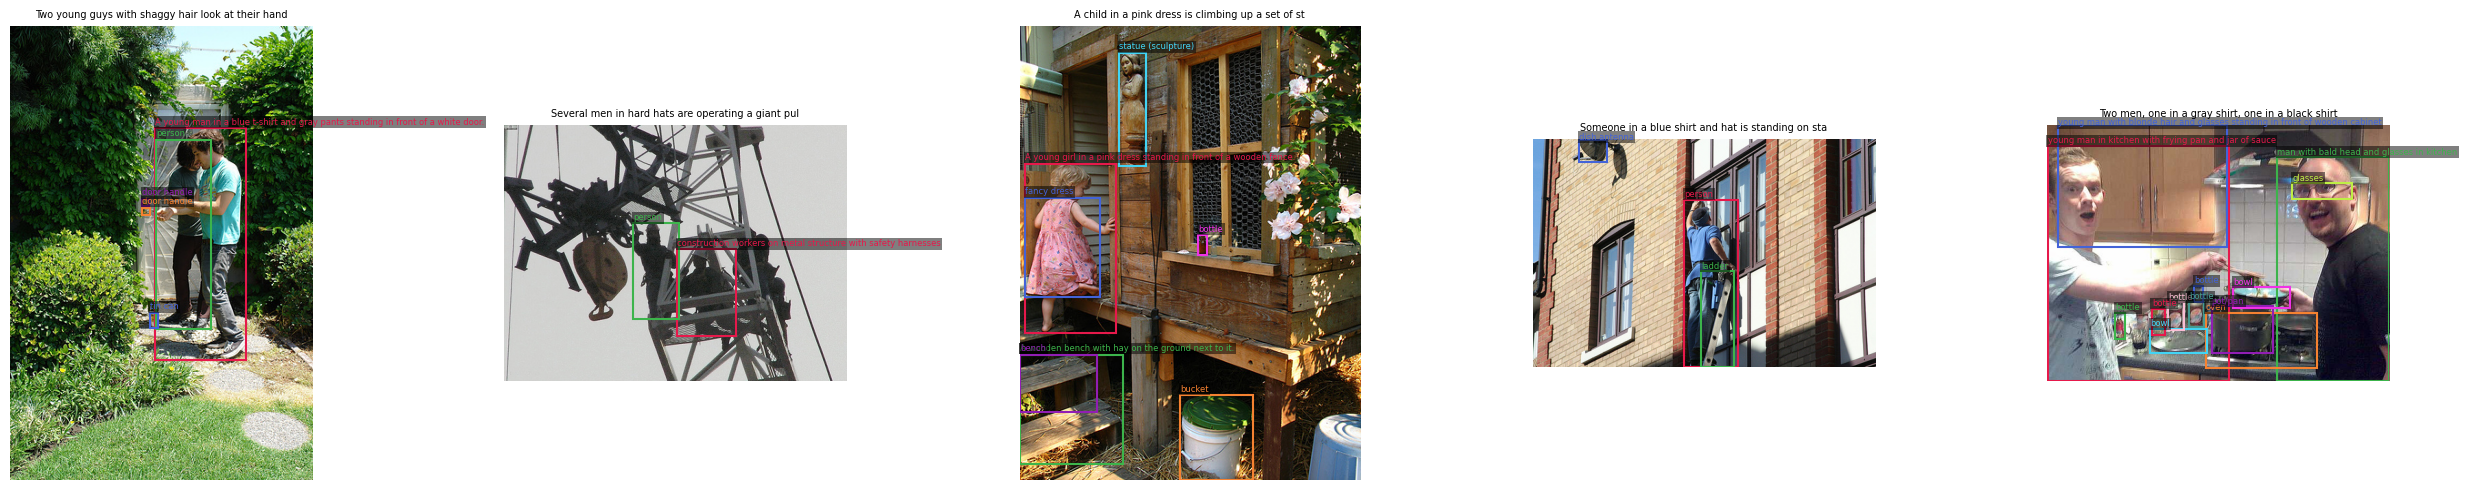
\includegraphics[width=\linewidth]{output.png}
    \caption{Florence-2 \texttt{<DENSE\_REGION\_CAPTION>} on five Flickr30k
    test images. Each coloured box is an auto-generated (bbox, label) pair,
    covering fine-grained entities across the scene.}
    \label{fig:florence2}
\end{figure}

\subsection{In Progress}

Training experiments for M$_\text{human}$ and M$_\text{auto}$ are currently
running on a Colab L4 GPU (23.7\,GB VRAM). Results are not yet available; the
frozen B0 baselines in Section~\ref{sec:findings} serve as the comparison floor.

%-----------------------------------------------------------------------
\section{Early Findings}
\label{sec:findings}
%-----------------------------------------------------------------------

We have completed benchmarking across all three evaluation metrics on frozen
baseline models. All results are on held-out validation sets.

\textbf{PASCAL VOC 2012 val --- zero-shot segmentation mIoU}
(\texttt{02d\_maskclip\_eval.ipynb}, \texttt{03\_siglip\_b0\_eval.ipynb}).

\begin{table}[h]
\centering
\small
\begin{tabular}{llcc}
\toprule
\textbf{Model} & \textbf{Method} & \textbf{Ours} & \textbf{Published} \\
\midrule
CLIP ViT-B/16   & Standard  & 8.46\%  & ---    \\
CLIP ViT-B/16   & MaskCLIP  & 19.90\% & 22.4\% \\
CLIP ViT-B/16   & SCLIP     & 14.01\% & 35.6\% \\
\midrule
SigLIP-B/16-384 & MaskCLIP (B0, frozen) & 1.43\% & --- \\
\bottomrule
\end{tabular}
\caption{VOC 2012 val mIoU. Published gaps reflect 336\,px input, prompt
ensembling, and PAMR post-processing not used here.}
\end{table}

\textbf{Flickr30k Pointing Game Accuracy}
(\texttt{06\_pointing\_game\_eval.ipynb}, 200 val images, 2,124 phrase--bbox pairs,
seed\,=\,42). For each pair we find the highest-scoring patch and check whether
its centre falls inside the GT bounding box.

\begin{table}[h]
\centering
\small
\begin{tabular}{lccc}
\toprule
\textbf{Model} & \textbf{Correct} & \textbf{Total} & \textbf{Accuracy} \\
\midrule
SigLIP-B/16-384 (frozen B0) & 313 & 2,124 & 14.74\% \\
\bottomrule
\end{tabular}
\caption{Flickr30k Pointing Game on 200 val images.}
\end{table}

Per-image accuracy is bimodal: best images (67--100\%) have 4--6 short concrete
phrases; worst images (0\%) have 12--19 abstract or whole-scene phrases.

\textbf{Flickr30k Recall@1 at IoU\,$\geq$\,0.5}
(\texttt{06\_pointing\_game\_eval.ipynb}, same 200 images). We select a set of
patches, form their tight bounding box in original image coordinates, and check
IoU $\geq$ 0.5 against the GT box. Three patch-selection strategies are evaluated.

\begin{table}[h]
\centering
\small
\begin{tabular}{llccc}
\toprule
\textbf{Model} & \textbf{Strategy} & \textbf{Hits} & \textbf{Total} & \textbf{R@1} \\
\midrule
SigLIP B0 (frozen) & top-10  & 145 & 2,124 & 6.83\% \\
SigLIP B0 (frozen) & top-25  & 168 & 2,124 & 7.91\% \\
SigLIP B0 (frozen) & halfmax & 161 & 2,124 & 7.58\% \\
\bottomrule
\end{tabular}
\caption{Flickr30k Recall@1 (IoU\,$\geq$\,0.5) on 200 val images. The halfmax
strategy selects all patches with similarity $\geq 0.5\times\max$ similarity.}
\end{table}

The drop from 14.74\% (pointing game) to $\sim$7\% (Recall@1) reveals that the
frozen model's top-$k$ patches are spatially scattered --- the argmax occasionally
lands in the right region, but the surrounding patches span the full image, causing
the predicted box to be too large and IoU to collapse. This confirms that SigLIP's
patch tokens carry almost no explicit phrase-grounding signal, which is precisely
the deficiency GRAFT targets. Published CLIP-based zero-shot phrase grounders
achieve 40--65\% Recall@1 on Flickr30k, leaving substantial headroom.

%-----------------------------------------------------------------------
\section{Revised Evaluation Design and Scope}
%-----------------------------------------------------------------------

\subsection{Evaluation Metrics}

\textbf{Primary --- Flickr30k Pointing Game and Recall@1 (IoU\,$\geq$\,0.5).}
Both metrics measure phrase-to-region alignment directly on held-out images ---
the same task the region loss trains. Any improvement from fine-tuning will appear
directly and unambiguously. Frozen B0 baselines (14.74\% and 6.83--7.91\%) are
near-chance, leaving large room for improvement.

\textbf{Guardrail --- PASCAL VOC 2012 mIoU.}
VOC mIoU is retained only as a sanity check, for two reasons. First, SigLIP is
pre-trained on billions of image--text pairs; 29k Flickr30k images will not
meaningfully shift class-level segmentation performance, and any change is likely
noise. Second, the tasks are categorically different: we train on noun phrase
grounding (``two young guys'', ``a red jacket'') while VOC tests semantic class
labelling (``aeroplane'', ``cat''). We use VOC only to confirm that fine-tuning
does not catastrophically destroy the frozen model's existing spatial structure.

\textbf{Dropped.} ImageNet-1K top-1, CIFAR-100, ARO, SugarCrepe, and Winoground
are descoped --- none are sensitive to the patch-level phrase grounding capability
this project targets.

\subsection{Revised Scope and Timeline}

The original proposal's three-stage pipeline (SCLIP region extraction $\to$
Qwen2-VL-2B captioning over CC3M $\to$ LoRA fine-tuning) is not feasible in the
remaining time. We propose a two-condition comparison that preserves the core
scientific question:

\begin{itemize}[leftmargin=1.5em, itemsep=1pt]
    \item \textbf{M$_\text{human}$}: fine-tuned on Flickr30k Entities human-annotated
    phrase--bbox pairs (upper-bound condition).
    \item \textbf{M$_\text{auto}$}: fine-tuned on Florence-2 auto-generated (bbox, label)
    pairs on the same images (self-supervised condition).
\end{itemize}

The minimal deliverable is a three-way table --- B0 vs.\ M$_\text{human}$ vs.\
M$_\text{auto}$ --- on Pointing Game and Recall@1, answering: does region-level
supervision improve phrase grounding, and does auto-generated supervision approach
human-annotated quality?

\textit{Week 1}: complete M$_\text{human}$, sweep $\tau$ and $\lambda$.
\textit{Week 2}: run Florence-2 annotation, train M$_\text{auto}$.
\textit{Week 3}: ablations and final write-up.

\end{document}
